\chapter{Visual Mappings And Interactive Functionality}
This chapter describes different visualizations and interaction methods developed based on the visualization requirements and data abstraction discussed in Chapter 2 and 4. In general, the visualization is divided into two parts: Session visualization which visualize movement in one particular session and Summary visualization which visualize movement over different sessions. Both visualization is organized in an application where user can select player and sessions he has played. At first, the earlier version of visualization will be explained. This earlier version is not used in the final version since it's difficult to get any information intuitively. Then, each type of visualization and its interaction used in the final version will be discuss. In the end, the application which encapsulate both visualization will be presented.

\section{Early version of the Visualization}
The first visualization method chosen to represent \ref{t11} and \ref{t12} is line chart. In this approach, the x area is shown as a horizontal axis and the number of events shown in vertical axis with the line signify the changes of number of events for different x area unit. In the log file, each event is recorded with distinct 3D coordinate location. The x value from this coordinate is a decimal, therefore visualizing each one of this x value will require a lot of space. To solve this, the events are then grouped by the rounded x value. In figure 5.1 below, Negative events are shown in red line and Positive events are shown in blue line. As we can see, it's possible which event type happened more in a certain x unit, however it is difficult to see how big a percentage is it compare to total number of events happened in the same x unit.

\begin{figure}
\centering
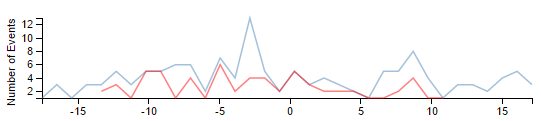
\includegraphics[width=100mm]{linechart.png}
\caption{First visualization version for \ref{t13} and \ref{t14} using Scatter Plot}
\end{figure}

\begin{figure}
\centering
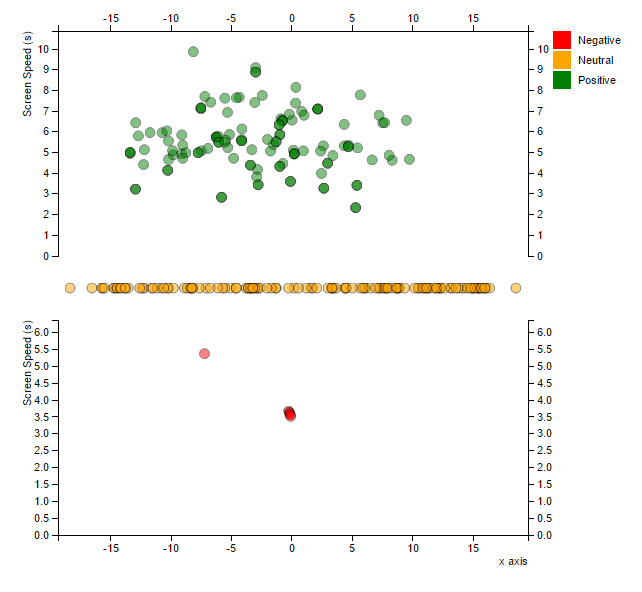
\includegraphics[width=100mm]{scatterplot.png}
\caption{First visualization version for \ref{t11} and \ref{t12} using Line Chart}
\end{figure}

Visualization method chosen to represent \ref{t13} and \ref{t14} is scatter plot. At first, each event type is presented in three different chart area: top are for Positive events, middle are for Neutral events, and bottom area for Negative events. Similar to the line chart, the x value from the 3D coordinate location are represented in horizontal x axis. However, the vertical axis here represent the screen speed. For the scatter plot, each event is shown as a plot in the chart area according to it's x value and screen speed as shown in figure 5.2. Even though similar pattern can be seen on the scatter plot, occlusion problem prevent users to know how many event are actually happened in a certain x area.

\section{Session Visualization}
The Session Visualization visualizes events within a game session. Basically, the requirement can be split into two: (i) knowing the distribution of events and movements (ii) knowing the distribution of events, movements and screen speed. Therefore, there are two chart developed to meets these requirements: stacked area for (i) and heatmap for (ii), each of which will be explain in details in this section.

\subsection{Stacked Graph}
Build on layered area graph, Stacked Graph is widely used to visualize evolution of variable over times such as document theme \cite{havre}, box office movie revenue\footnote{\url{http://www.nytimes.com/interactive/2008/02/23/movies/20080223_REVENUE_GRAPHIC.html?_r=0}}, listening history in Last.fm \cite{byron},etc., Stacked Graph is chosen because its ability to show individual value of a variable, the difference between values of different variables as well as the total of overall value. In my approach, instead of using this metaphor to show evolution over time, it is used to show distribution of events over spatial coordinate \ref{t11}\ref{t12} as shown in figure 5.3. Here, the horizontal axis represents x coordinate and vertical axis represents number of events. Each event type is represented as an area with different color: Red (Negative), Yellow (Neutral), and Green (Positive). To help user understand better the distribution of each event type, different layout of stacked graph is provided: 
\begin{enumerate}
  \item Linear: zero y axis is used as the baseline, with the stack ordered from bottom as negative, neutral, positive.
  \item Silhouette: the graph is centered as in streamgraphs.
  \item Positive: zero y axis is located at the top of the chart and is used as the baseline with the stack ordered from top as positive, neutral, negative.
  \item Neutral-Negaive: zero y axis is located in the middle of the chart. Neutral and Positive event is shown on the positive area of y axis and Negative is shown on the negative area of y axis.
  \item Positive-Neutral: zero y axis is located in the middle of the chart. Positive event is shown on the positive area of y axis, while Neutral and Negative is shown on the negative area of y axis.
\end{enumerate}

\begin{figure}
\centering
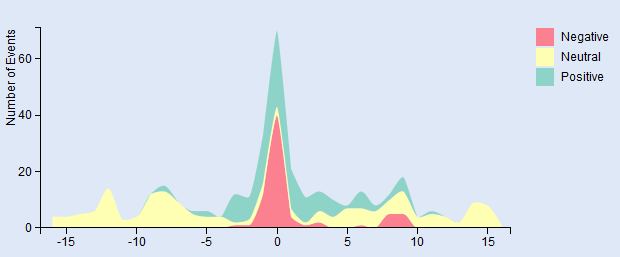
\includegraphics[width=100mm]{stackedgraph_linear.png}
\caption{Stacked Graph with Linear Layout}
\end{figure}

\begin{figure}[htp] % not h only
\centering
\subfloat[Silhouette]{%
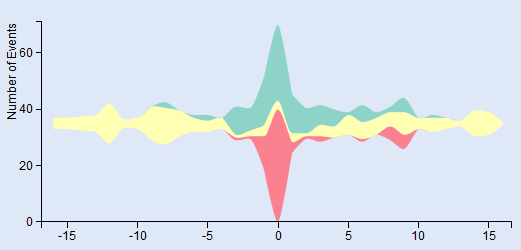
\includegraphics[width=0.4\textwidth]{stackedgraph_silhouette.png}%
\label{fig:silhouette}%
}\hfil
\subfloat[Positive]{%
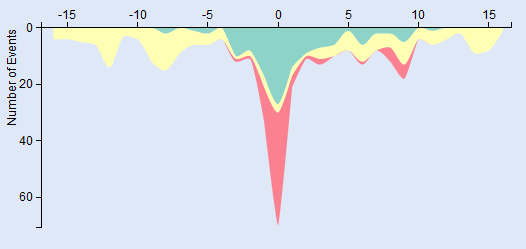
\includegraphics[width=0.4\textwidth]{stackedgraph_positive.png}%
\label{fig:positive}%
}

\subfloat[Neutral-Negative]{%
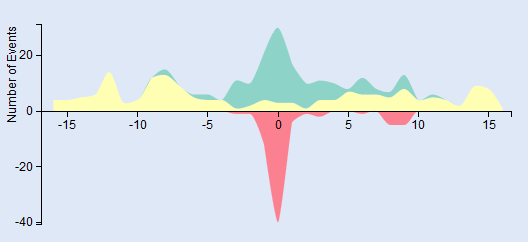
\includegraphics[width=0.4\textwidth]{stackedgraph_neutral_neg.png}%
\label{fig:neutral-negative}%
}\hfil
\subfloat[Positive-Neutral]{%
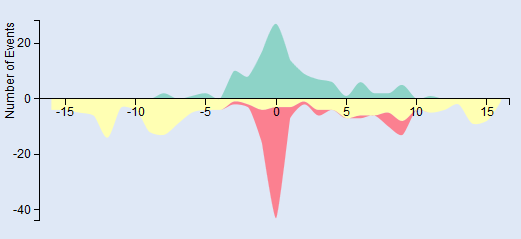
\includegraphics[width=0.4\textwidth]{stackedgraph_positive_neutral.png}%
\label{fig:positive-neutral}%
}

\caption{Different Layout of the Stacked Graph representing number of events over x-axis}
\end{figure}

For each stacked graph layout, user can choose which object type to show on the graph \ref{t15}. Options are available as radio button on top of the chart. Therefore, choosing Bonus will show only Positive and Neutral events, choosing Obstacle will show only Neutral and Negative events, and choosing Enemy will show all event type.

\subsection{Heat Map}
Heat Map is a quite popular visualization method nowadays due to its ability which allows user to see variable with the highest value at one glance. Most of the time, heatmap is implemented on geographical map to represent variable value over certain area on map, i.e: Natural Disaster Risk by Location\footnote{\url{http://www.rms.com/}}, population density\footnote{\url{https://en.wikipedia.org/wiki/Population_density}}, Number of picture taken in an area\footnote{\url{http://sightsmap.com/}}, etc. Heat map is also used to track eye movement or mouse click on a website, and representing DNA microarray data in the form of cluster heat map\cite{friendly}. Heat map uses color gradation to represent the hotness level of a variable. Usually, red color is used to represent the high value (hot) and blue is used to represent the low value (cold). However, other color combination can also be used. To represent distribution of events and screen speed over x axis \ref{t13}\ref{t14}, the events are first grouped based on it's x value and normalized screen speed. The number of events is then represented as heat map on the graph with highest number of events in red color. Normalized screen speed is represented as vertical axis and x value is represented as horizontal axis. Using the same approach used in scatter plot chart, each event type is presented in different area: top for positive, middle for neutral, and bottom for negative. For Neutral events, the screen speed is not calculated since it basically mean an object has been avoided or missed. For Negative events, the screen speed is represented in negative to show that it's an uncalculated movement. For the heatmap, user can also choose to show a specific object \ref{t16} by clicking the radio button associated with the desired object.

\begin{figure}
\centering
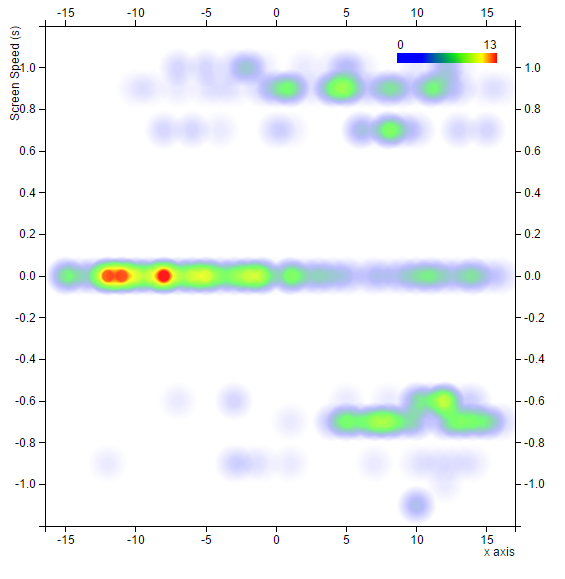
\includegraphics[width=110mm]{heatmap.png}
\caption{Heatmap}
\end{figure}


\section{Summary Visualization}
\subsection{Visualization by x-area}
\begin{figure}
\centering
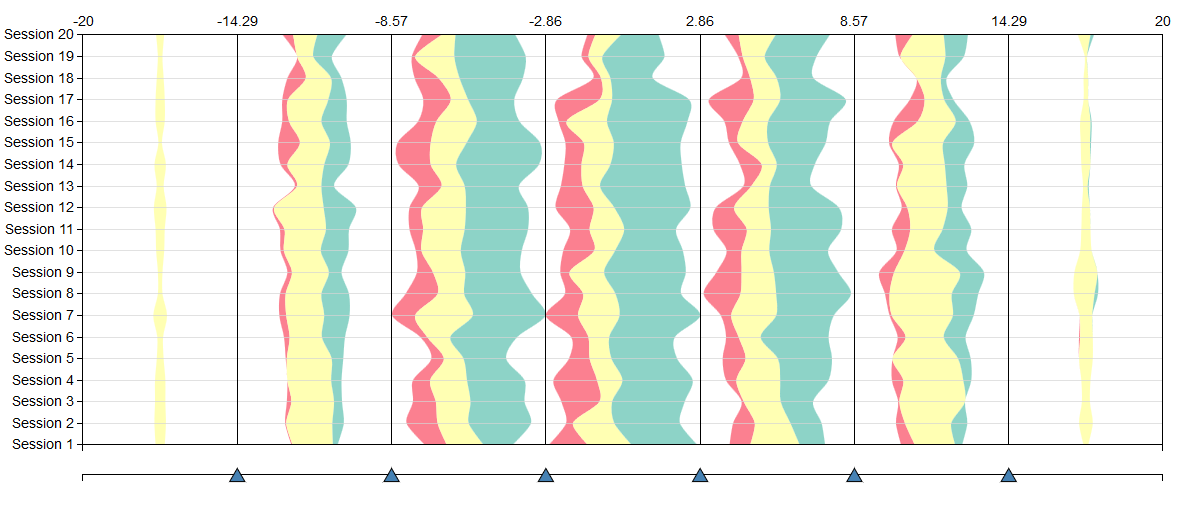
\includegraphics[width=130mm]{summary_type1.png}
\caption{Summary Chart divided by range of x-area}
\end{figure}

\subsection{Visualization by number of events}
\begin{figure}
\centering
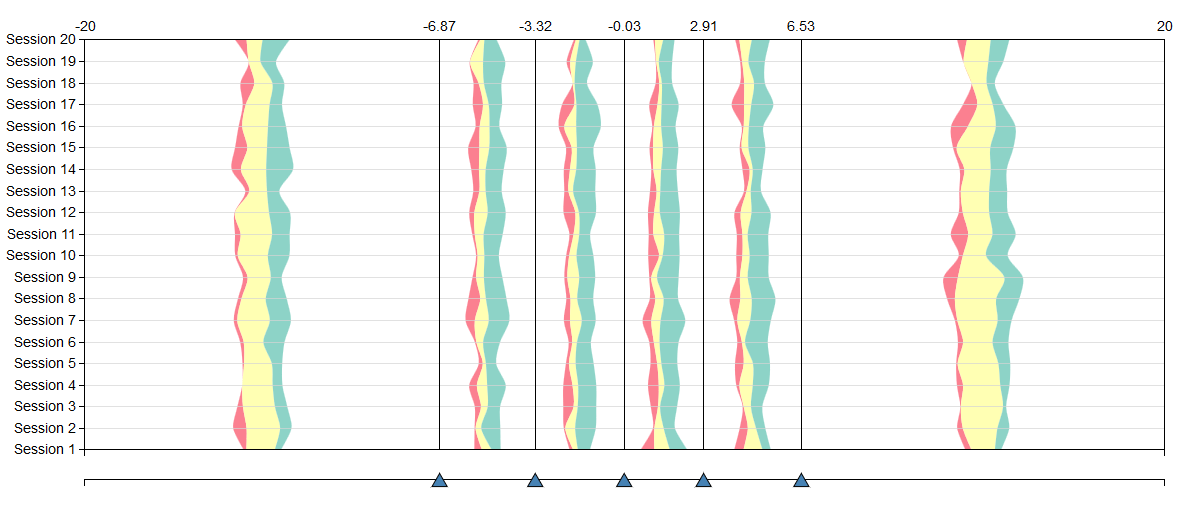
\includegraphics[width=130mm]{summary_type2.png}
\caption{Summary Chart divided by number of events}
\end{figure}

\subsection{Interaction Technique}
==Event Type
==Slider
==Sliding the line
\begin{figure}
\centering
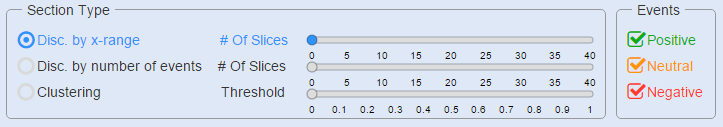
\includegraphics[width=130mm]{interaction_bar.png}
\caption{Interaction Bar for Summary Visualization}
\end{figure}
\section{General Interface}
Both the Session and Summary visualization are..
\begin{figure}
\centering
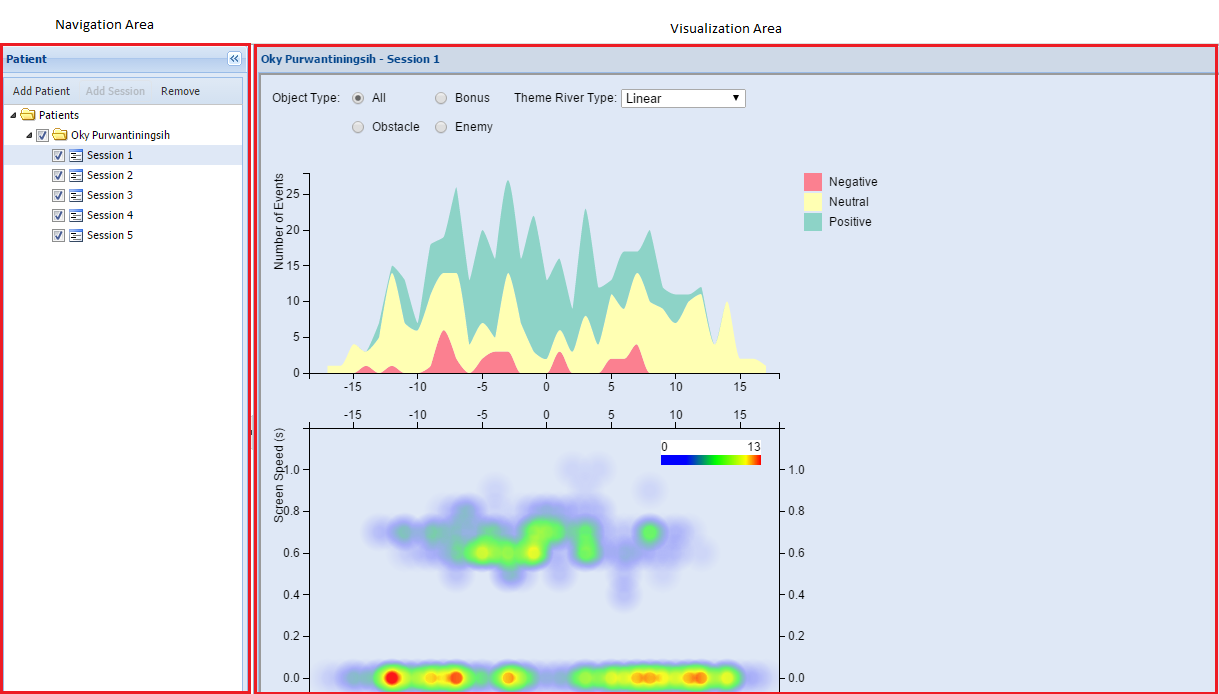
\includegraphics[width=130mm]{interface_app.png}
\caption{Application Interface}
\end{figure}